\chapter{Table of Profiles} % Main chapter title

\label{Chapter6} 

While in related work I examined load profiling in general,
this chapter focuses on how data in load profiles is presented.  
It can be portrayed in various shapes and forms,
using all kinds of attributes and features to do so. 
First, main load profiling features will be defined.
Second, using these features a general load profile table will be constructed.
Third, references from related work and use cases will be mapped to the table.
Using this information main features will be selected.
Fourth, using a reduced feature set a more detailed table will be formed.
Again, the table will be populated using the same references as before.
Finally, using this information a research direction will be formed.

\section{Feature Set} \label{sec:feature_set}

Using related work and use case references,
we can extract the most commonly used features to portray load profiles.

\begin{outline}
    \1 power
    \1 time
    \1 operating time (how long appliance or appliances is turned on)
    \1 appliances (a set)
    \1 Number of activations (How many times appliance or appliances were turned on)
\end{outline}

\section{General table}
Using these features we can form a table with all possible combinations.
Some combinations do not make logical sense and the others repeat themselves.
Combinations marked with X are such examples.
Table \ref{tab:general_map} is then populated with references from previous chapters.

\begin{table}[H]
    \caption{General table of load profiles}
    \label{tab:general_map}
    \begin{tabular}{|l|l|l|l|l|l|}
    \hline
        &
        frequency &
        appliances &
        \begin{tabular}[c]{@{}l@{}}number of\\ activations\end{tabular} &
        \begin{tabular}[c]{@{}l@{}}power\\ (avg)\end{tabular} &
        \begin{tabular}[c]{@{}l@{}}operating\\ time\end{tabular} \\ \hline
    appliances                                                      &   & X & X & X  & X    \\ \hline
    \begin{tabular}[c]{@{}l@{}}number of\\ activations\end{tabular} & X &   & X & X  & X    \\ \hline
    \begin{tabular}[c]{@{}l@{}}power \\ (avg)\end{tabular}          & X & 1 &   & X  & X    \\ \hline
    \begin{tabular}[c]{@{}l@{}}power \\ (array)\end{tabular}        & 1 & X & X & X  & X    \\ \hline
    \begin{tabular}[c]{@{}l@{}}power \\ (histogram)\end{tabular}    &   &   & X & X  & X    \\ \hline
    \begin{tabular}[c]{@{}l@{}}operating\\ time\end{tabular}        & X & 1 &   &    & X    \\ \hline
    time array                                                      & X & X & 1 & 21 & 1(3) \\ \hline
    \end{tabular}
\end{table}

Based on table \ref{tab:general_map} it is possible to see that the most commonly
published feature combination is time and power. This combination will be used 
as a baseline when making a more detailed table. Although the operating time feature was 
explored in a few publications a bit, and it seems quite promising, we are 
focusing on activation-based histogram representation.
Based on table \ref{tab:general_map} it is possible to see that not much attention was given to it. 

\section{Detailed table}

This section will focus on exploring possible load profiles using activation-based histogram representation,
while using the power feature as a baseload. 
Features from \ref{tab:general_map} will be explored in higher detail. 
They will be split and arranged in a way that all 21 publications and power-based presentations will be divided into as many groups as possible. 
This should expose possible activation-based profiles as well as unpublished power-based profiles.

\subsection{Sub-features} \label{sec:subfeatures}

Main features were already described in section \ref{sec:feature_set}.
It is possible to further divide them into smaller so-called sub-features.
These are reshaped and grouped as follows:
\begin{outline}

\1 Way of presenting a profile
\2 Per-house load profile
\2 Per-appliance load profiles
\2 Per-house and per appliance load profile

\1 By time range of profile 
\2 Daily
\2 Weekly
\2 Monthly
\2 Yearly

\1 Way of measuring usage
\2 Average power use 
\2 Activation or frequency of activation
\2 Operating time
\end{outline}

\subsection{Sketches of load profiles}
A most common way load profiles are presented is a daily power consumption profile such as shown in figure \ref{fig:daily_power_profile}. 
The graph is a sketch, but it represents a standard load profile with morning and evening peaks.

\begin{figure}[H]
	\centering
	\caption{"Average daily usage profile for an appliance or a building"}
	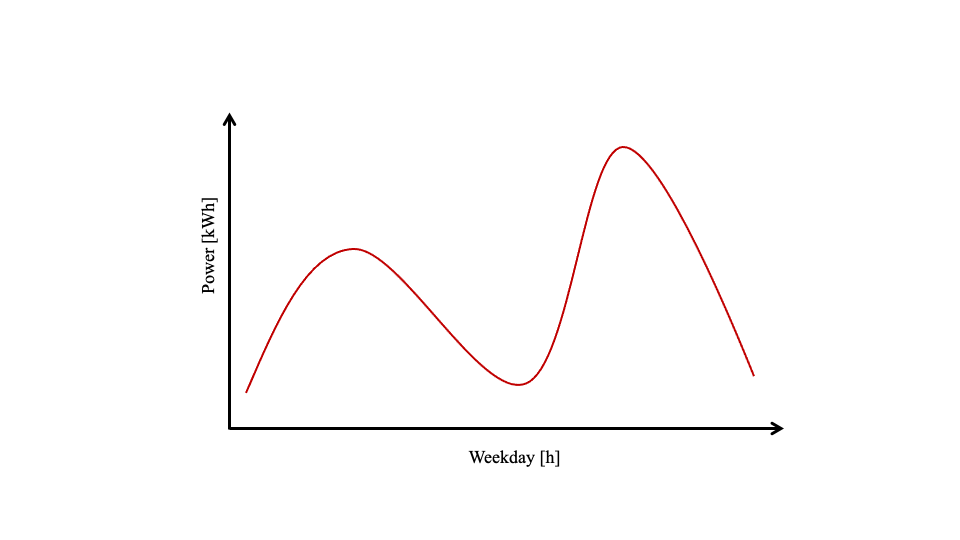
\includegraphics[width=0.9\textwidth]{Figures/profile_sketches/Slide1.png}
	\label{fig:daily_power_profile}
\end{figure}

Some references include daily usage profiles as a histogram of activation at a point in a day, such as a figure \ref{fig:daily_act_profile}.

\begin{figure}[H]
	\centering
	\caption{"Histogram of daily activations profile for an appliance or a building"}
	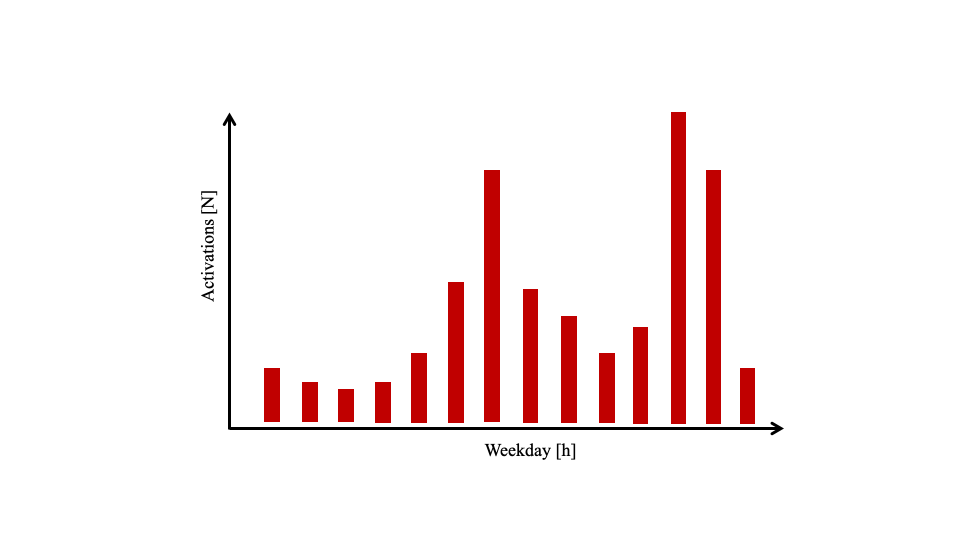
\includegraphics[width=0.9\textwidth]{Figures/profile_sketches/Slide5.png}
	\label{fig:daily_act_profile}
\end{figure}

All figures can present whole-house usage or per-device usage. Each presentation has its pros and cons. 
To present more information sub-meter data can be used to represent whole-house usage with per-appliance contributions.
Such as on figure \ref{fig:daily_act_m_profile} and \ref{fig:daily_power_m_profile}.

\begin{figure}[H]
	\centering
	\caption{"Histogram of daily activations profile for an appliance A and B"}
	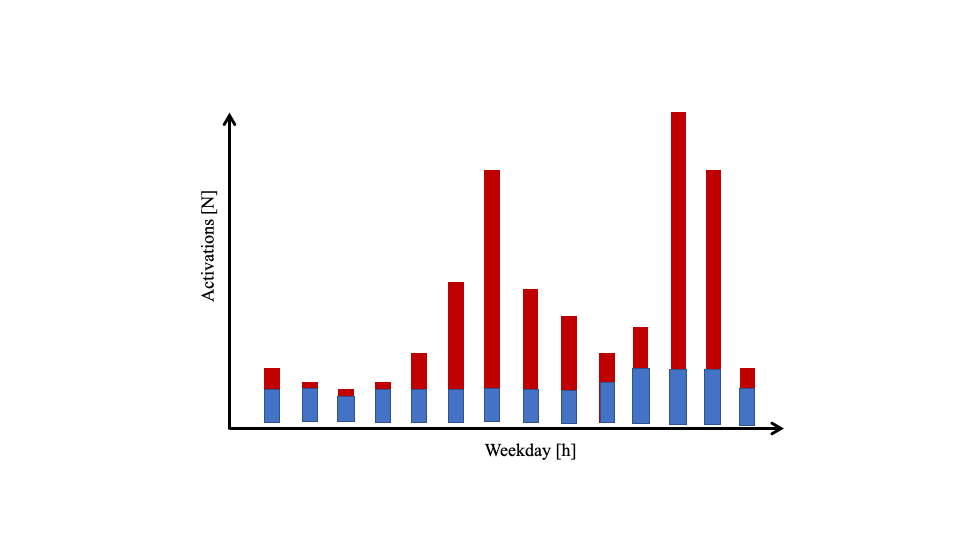
\includegraphics[width=0.9\textwidth]{Figures/profile_sketches/Slide8.png}
	\label{fig:daily_act_m_profile}
\end{figure}
\begin{figure}[H]
	\centering
	\caption{"Average weekday power consumption for appliances A, B and C"}
	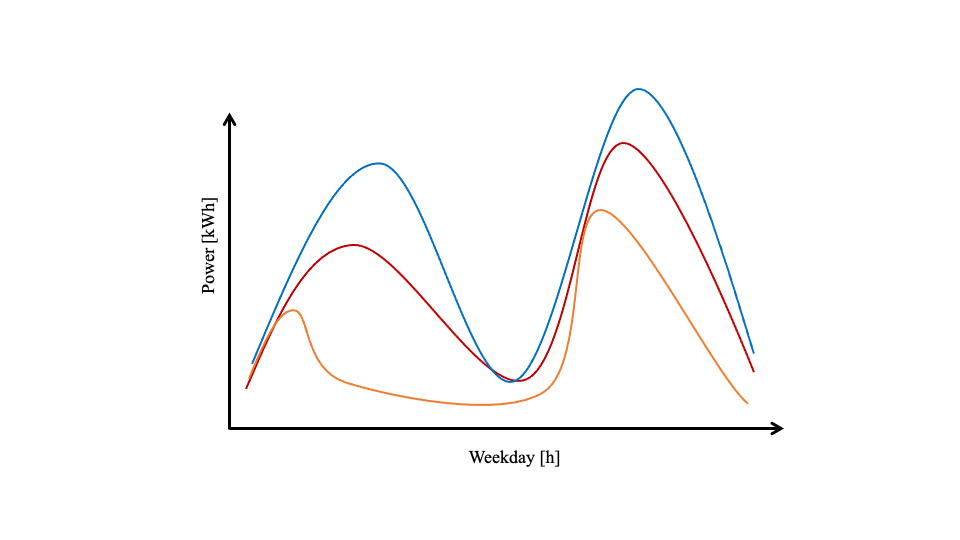
\includegraphics[width=0.9\textwidth]{Figures/profile_sketches/Slide2.png}
	\label{fig:daily_power_m_profile}
\end{figure}

To present as much information as possible all above-mentioned attributes 
can be presented in a multidimensional way such as heatmap in a way shown in figure \ref{fig:heatmap_2dtime} and \ref{fig:heatmap_all_appl}.

\begin{figure}[H]
	\centering
	\caption{"Number of daily activations / power consumption of one appliance / house in one month period"}
	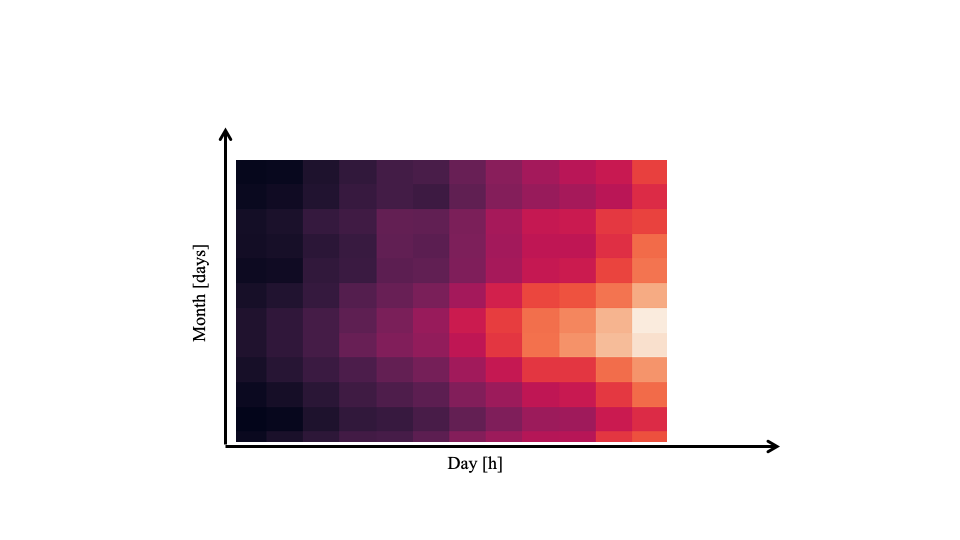
\includegraphics[width=0.9\textwidth]{Figures/profile_sketches/Slide10.png}
	\label{fig:heatmap_2dtime}
\end{figure}
\begin{figure}[H]
	\centering
	\caption{"Number of activations / power consumption for each appliance in one month period"}
	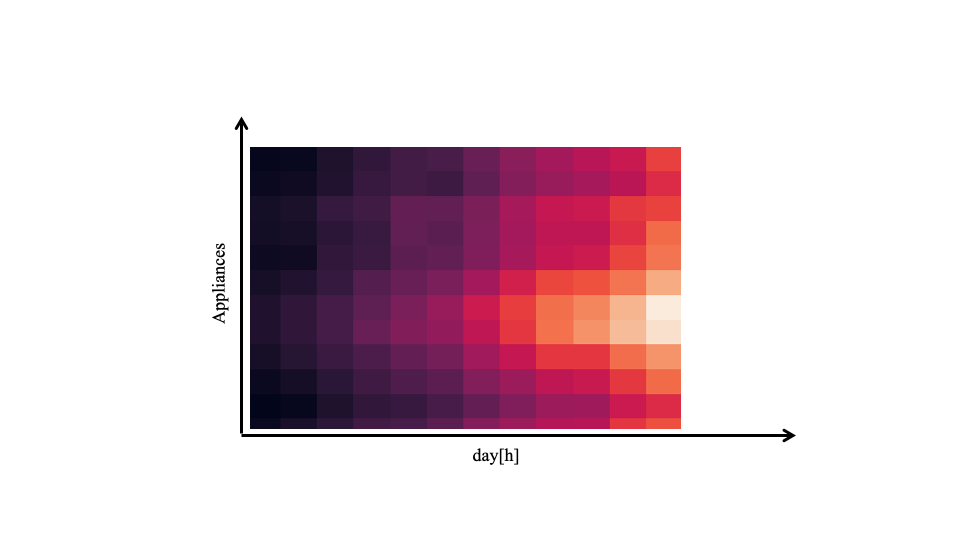
\includegraphics[width=0.9\textwidth]{Figures/profile_sketches/Slide12.png}
	\label{fig:heatmap_all_appl}
\end{figure}

\subsection{Table of combinations or detailed table}

The above-shown profiles can be combined, yielding a new way of displaying the data.
Bellow, a map with combinations of the above-mentioned profiles is presented. 
The purpose of table \ref{fig:map_fig} to generate and show possible combinations.
Some combinations that had similar output were grouped, and some that could not be sketched were discarded. 

\begin{figure}[H]
	\centering
	\caption{"Table of combinations"}
	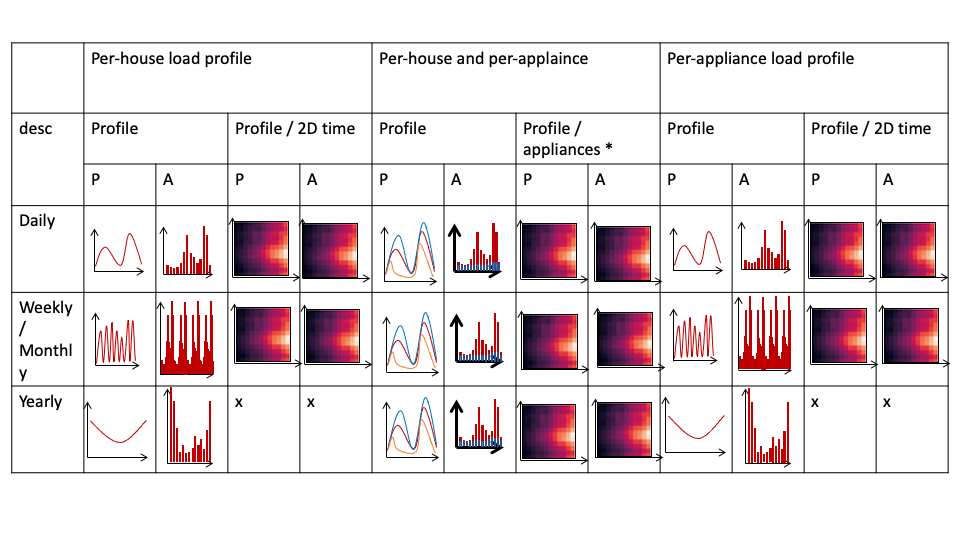
\includegraphics[width=0.9\textwidth]{Figures/profile_sketches/Slide14.png}
	\label{fig:map_fig}
\end{figure}

Figure above \ref{fig:map_fig}, uses sub-features from previous subsection \ref{sec:subfeatures}. 
In general, the table is formatted in a way that features from columns are
used in the x-axis of a plot, and rows are used in the y or z-axis of a plot. 

The column of the table presents the time domain. \"Daily\" means that the load profile presents
average usage for one day, weekly means it presents usage for a week.
To be clear, for one to construct a decent daily profile, one needs a few
weeks of data. The same goes for yearly profiles, in that case, one needs many years' worth of data. 

The top row of the table is composed of 3 main groups. 
The first group focuses on per-house energy consumption.
The second group examines the energy consumption of each appliance in a house separately.
Third group analyses all appliances in a building.

The next row of the table is further divided into two groups. First is the profile group
which presents the given usage unit on the y-axis and time on the x-axis. 
Next is a profile with a time group. 
In this case, we present the given usage unit on the z-axis and then time on the x and y-axis.
Here, the second-time dimension can be anything from a week to a year.
In the case of the per-house subgroup includes appliances instead of time. 
Example for this is figure \ref{fig:heatmap_all_appl}.
The last columns present the usage unit, that is power (P) or a number of activations (A).

\subsection{Mapping references to the table of profiles}

To find useful load profiles, references from related work must be mapped.

\begin{table}[H]
	\caption{Table presents previously mentioned load profiles}
	\label{tab:contributions}

	\begin{tabular}{|l|cccc|cccc|cccc|}
	\hline
	Description                                                   & \multicolumn{4}{c|}{Per-house}                                                                                               & \multicolumn{4}{c|}{Per-appliance}                                                                                           & \multicolumn{4}{c|}{\begin{tabular}[c]{@{}c@{}}Per-house\\ per-appliance\end{tabular}}                                                         \\
																 & \multicolumn{2}{c|}{LP}                         & \multicolumn{2}{c|}{\begin{tabular}[c]{@{}c@{}}2D \\ time LP\end{tabular}} & \multicolumn{2}{c|}{LP}                         & \multicolumn{2}{c|}{\begin{tabular}[c]{@{}c@{}}2D\\  time LP\end{tabular}} & \multicolumn{2}{c|}{LP}                               & \multicolumn{2}{c|}{\begin{tabular}[c]{@{}c@{}}Appliances\\ side by side\end{tabular}} \\ \cline{1-1}
	\begin{tabular}[c]{@{}l@{}}Range of time\\ axis\end{tabular} & \multicolumn{1}{c|}{P} & \multicolumn{1}{c|}{A} & \multicolumn{1}{c|}{P}                         & A                         & \multicolumn{1}{c|}{P} & \multicolumn{1}{c|}{A} & \multicolumn{1}{c|}{P}                         & A                         & \multicolumn{1}{c|}{P}    & \multicolumn{1}{c|}{A}    & \multicolumn{1}{c|}{P}                               & A                               \\ \hline
	Daily                                                        & \multicolumn{1}{c|}{\begin{tabular}[c]{@{}c@{}} \citeyear*{Chuan2014} \\ \citeyear*{Csoknyai2019} \\ \citeyear*{H0} \\ \citeyear*{KAVOUSIAN2013184} \\ \citeyear*{CAPASSO1994} \\ \citeyear*{WALKER1985} \\ \citeyear*{GERBEC2005} \\ \citeyear*{Gao2018} \\ \citeyear*{Jeong2021} \\ \citeyear*{Joana2012} \\ \citeyear*{DER_heatmap_profile} \end{tabular}}  & \multicolumn{1}{c|}{}  & \multicolumn{1}{c|}{\begin{tabular}[c]{@{}l@{}} \citeyear*{2D_year_day_LP} \\ \citeyear*{Park2019} \\ \citeyear*{DER_heatmap_profile} \end{tabular}}   &    & \multicolumn{1}{c|}{\begin{tabular}[c]{@{}l@{}} \citeyear*{NILMAD2019} \\ \citeyear*{NILMAD22019} \\ \citeyear*{Issi2018} \\ \citeyear*{NILMAD2021} \\ \citeyear*{Castangia2021} \\ \citeyear*{occupancy2013}	\end{tabular}}  & \multicolumn{1}{c|}{\citeyear*{UKDALE}}  & \multicolumn{1}{c|}{}   &  \multicolumn{1}{c|}{}   & \multicolumn{1}{c|}{\begin{tabular}[c]{@{}l@{}} \citeyear*{Chuan2014} \\ \citeyear*{CAPASSO1994} \\ \citeyear*{Gao2018} 	\end{tabular}}   & \multicolumn{1}{c|}{}     & \multicolumn{1}{c|}{}      &    \\ \hline
	\begin{tabular}[c]{@{}l@{}}Weekly/\\ Monthly\end{tabular}    & \multicolumn{1}{c|}{\begin{tabular}[c]{@{}c@{}} \citeyear*{Csoknyai2019} \\ \citeyear*{H0} \\ \citeyear*{KAVOUSIAN2013184} \end{tabular}}  & \multicolumn{1}{c|}{}  & \multicolumn{1}{c|}{}                          &                           & \multicolumn{1}{c|}{}  & \multicolumn{1}{c|}{}  & \multicolumn{1}{c|}{}                          &                           & \multicolumn{1}{c|}{\citeyear*{weekly_per_appliance_LP}}    & \multicolumn{1}{c|}{}     & \multicolumn{1}{c|}{}                                &                                 \\ \hline
	Yearly                                                       & \multicolumn{1}{c|}{\begin{tabular}[c]{@{}c@{}} \citeyear*{Csoknyai2019} \\ \citeyear*{H0} \\ \citeyear*{KAVOUSIAN2013184} \end{tabular}}  & \multicolumn{1}{c|}{}  & \multicolumn{1}{c|}{}                          &                           & \multicolumn{1}{c|}{}  & \multicolumn{1}{c|}{}  & \multicolumn{1}{c|}{}                          &                           & \multicolumn{1}{c|}{}     & \multicolumn{1}{c|}{}     & \multicolumn{1}{c|}{}                                &                                 \\ \hline
	\end{tabular}
\end{table}

As can be seen from table \ref{tab:contributions}, most of the work (14 publications) has been done with standard daily load profiles with
per-house power usage such as figure \ref{fig:daily_power_profile}. 
Quite a lot of work (6 publications) has been done with per appliance daily power profiles.
A few publications were based on weekly and yearly load profiles,
a few used two-dimensional time and power presentation.
Only one publication found used activation and time-based histogram such as 
shown in figure \ref{fig:daily_act_profile}. During the research I focused on publications
from minority classes, meaning not all existing publications for standard load profiles are included. 
The purpose of table \ref{tab:contributions} is to present missing scientific contributions and patterns of publications.  

\subsection{Mapping use-cases to the table of combinations}

Table \ref{tab:use_cases} includes arranged publications from chapter \ref{Chapter5}. 
Similar pattern emerged as in table \ref{tab:contributions}. 

\begin{table}[H]
	\caption{Table presents references mentioned in use cases chapter}
	\label{tab:use_cases}
	\begin{tabular}{|l|cccc|cccc|cccc|}
	\hline
	Description &
	  \multicolumn{4}{c|}{Per-house} &
	  \multicolumn{4}{c|}{Per-appliance} &
	  \multicolumn{4}{c|}{\begin{tabular}[c]{@{}c@{}}Per-house\\ per-appliance\end{tabular}} \\
	 &
	  \multicolumn{2}{c|}{LP} &
	  \multicolumn{2}{c|}{\begin{tabular}[c]{@{}c@{}}2D \\ time LP\end{tabular}} &
	  \multicolumn{2}{c|}{LP} &
	  \multicolumn{2}{c|}{\begin{tabular}[c]{@{}c@{}}2D\\  time LP\end{tabular}} &
	  \multicolumn{2}{c|}{LP} &
	  \multicolumn{2}{c|}{\begin{tabular}[c]{@{}c@{}}Appliances\\ side by side\end{tabular}} \\ \cline{1-1}
	\begin{tabular}[c]{@{}l@{}}Range of time\\ axis\end{tabular} &
	  \multicolumn{1}{c|}{P} &
	  \multicolumn{1}{c|}{A} &
	  \multicolumn{1}{c|}{P} &
	  A &
	  \multicolumn{1}{c|}{P} &
	  \multicolumn{1}{c|}{A} &
	  \multicolumn{1}{c|}{P} &
	  A &
	  \multicolumn{1}{c|}{P} &
	  \multicolumn{1}{c|}{A} &
	  \multicolumn{1}{c|}{P} &
	  A \\ \hline
	Daily &
	  \multicolumn{1}{c|}{\begin{tabular}[c]{@{}c@{}} \citeyear*{energy_saving1} \\ \citeyear*{energy_saving3} \\ \citeyear*{EV2020} \\ \citeyear*{energyStealing2018} \\ \citeyear*{shift2015} \\ \citeyear*{optimiseCostShift2015} \\ \citeyear*{controll2014} \end{tabular}} &
	  \multicolumn{1}{c|}{} &
	  \multicolumn{1}{c|}{} &
	   &
	  \multicolumn{1}{c|}{\begin{tabular}[c]{@{}c@{}} \citeyear*{EV2020} \\ \citeyear*{elder1} \\ \citeyear*{elder2} \\   \citeyear*{occupancy2013}	  \end{tabular}} &
	  \multicolumn{1}{c|}{} &
	  \multicolumn{1}{c|}{} &
	   &
	  \multicolumn{1}{c|}{\citeyear*{Chuan2014}	 } &
	  \multicolumn{1}{c|}{} &
	  \multicolumn{1}{c|}{} &
	   \\ \hline
	\begin{tabular}[c]{@{}l@{}}Weekly/\\ Monthly\end{tabular} &
	  \multicolumn{1}{c|}{\begin{tabular}[c]{@{}c@{}} \citeyear*{energy_saving3} \\ \citeyear*{KAVOUSIAN2013184}  \end{tabular}} &
	  \multicolumn{1}{c|}{} &
	  \multicolumn{1}{c|}{} &
	   &
	  \multicolumn{1}{c|}{} &
	  \multicolumn{1}{c|}{} &
	  \multicolumn{1}{c|}{} &
	   &
	  \multicolumn{1}{c|}{} &
	  \multicolumn{1}{c|}{} &
	  \multicolumn{1}{c|}{} &
	   \\ \hline
	Yearly &
	  \multicolumn{1}{c|}{\begin{tabular}[c]{@{}c@{}}\citeyear*{energy_saving3}\end{tabular}} &
	  \multicolumn{1}{c|}{} &
	  \multicolumn{1}{c|}{} &
	   &
	  \multicolumn{1}{c|}{} &
	  \multicolumn{1}{c|}{} &
	  \multicolumn{1}{c|}{} &
	   &
	  \multicolumn{1}{c|}{} &
	  \multicolumn{1}{c|}{} &
	  \multicolumn{1}{c|}{} &
	   \\ \hline
	\end{tabular}
\end{table}

\subsection{Table of use case groups}

Table \ref{tab:groups} presents same publications as \ref{tab:use_cases},
but only group names are shown.
The table indicates how groups are arranged.
Where anomaly detection and elderly care are dominating in the per-appliance part of the table,
energy-saving and grid management are dominating in a per-house part of the table. 

\begin{table}[H]
    \caption{Table presents references mentioned in use cases chapter}
	\label{tab:groups}
    \begin{adjustbox}{width=1.2\textwidth,center=\textwidth} 
        \begin{tabular}{|l|cccc|cccc|cccc|}
            \hline
            \begin{tabular}[c]{@{}l@{}}ES - energy saving\\ GM - grid management\\ AD - anomaly detection\\ EC - elderly care\\ X - unfeasible\end{tabular} &
              \multicolumn{4}{c|}{Per-house} &
              \multicolumn{4}{c|}{Per-appliance} &
              \multicolumn{4}{c|}{\begin{tabular}[c]{@{}c@{}}Per-house\\ per-appliance\end{tabular}} \\ \cline{2-13} 
             &
              \multicolumn{2}{c|}{LP} &
              \multicolumn{2}{c|}{\begin{tabular}[c]{@{}c@{}}2D \\ time LP\end{tabular}} &
              \multicolumn{2}{c|}{LP} &
              \multicolumn{2}{c|}{\begin{tabular}[c]{@{}c@{}}2D\\  time LP\end{tabular}} &
              \multicolumn{2}{c|}{LP} &
              \multicolumn{2}{c|}{\begin{tabular}[c]{@{}c@{}}Appliances\\ side by side\end{tabular}} \\ \hline
            \begin{tabular}[c]{@{}l@{}}Range of time\\ axis\end{tabular} &
              \multicolumn{1}{c|}{P} &
              \multicolumn{1}{c|}{A} &
              \multicolumn{1}{c|}{P} &
              A &
              \multicolumn{1}{c|}{P} &
              \multicolumn{1}{c|}{A} &
              \multicolumn{1}{c|}{P} &
              A &
              \multicolumn{1}{c|}{P} &
              \multicolumn{1}{c|}{A} &
              \multicolumn{1}{c|}{P} &
              A \\ \hline
            Daily &
              \multicolumn{1}{c|}{ES, GM} &
              \multicolumn{1}{c|}{} &
              \multicolumn{1}{c|}{} &
               &
              \multicolumn{1}{c|}{\begin{tabular}[c]{@{}c@{}}AD, EC,\\ ES\end{tabular}} &
              \multicolumn{1}{c|}{} &
              \multicolumn{1}{c|}{} &
               &
              \multicolumn{1}{c|}{GM} &
              \multicolumn{1}{c|}{} &
              \multicolumn{1}{c|}{} &
               \\ \hline
            \begin{tabular}[c]{@{}l@{}}Weekly/\\ Monthly\end{tabular} &
              \multicolumn{1}{c|}{ES} &
              \multicolumn{1}{c|}{} &
              \multicolumn{1}{c|}{} &
               &
              \multicolumn{1}{c|}{} &
              \multicolumn{1}{c|}{} &
              \multicolumn{1}{c|}{} &
               &
              \multicolumn{1}{c|}{} &
              \multicolumn{1}{c|}{} &
              \multicolumn{1}{c|}{} &
               \\ \hline
            Yearly &
              \multicolumn{1}{c|}{ES} &
              \multicolumn{1}{c|}{} &
              \multicolumn{1}{c|}{X} &
              X &
              \multicolumn{1}{c|}{} &
              \multicolumn{1}{c|}{} &
              \multicolumn{1}{c|}{X} &
              X &
              \multicolumn{1}{c|}{} &
              \multicolumn{1}{c|}{} &
              \multicolumn{1}{c|}{} &
               \\ \hline
            \end{tabular}
    \end{adjustbox} 
    \end{table}

The figures listed above clearly depict the void not filled by publications. 
Although they may not be published, they still have a possible use case. 
In table \ref{tab:groups_proposed} empty spaces are filled 
with possible use cases for given load profiles. 

\begin{table}[H]
    \caption{"Proposed use cases for profiles"}
    \label{tab:groups_proposed}
    \begin{adjustbox}{width=1.2\textwidth,center=\textwidth} 
    \begin{tabular}{|l|cccc|cccc|cccc|}
    \hline
    \begin{tabular}[c]{@{}l@{}}ES - energy saving\\ GM - grid management\\ AD - anomaly detection\\ EC - elderly care\\ X - unfeasible\end{tabular} &
      \multicolumn{4}{c|}{Per-house} &
      \multicolumn{4}{c|}{Per-appliance} &
      \multicolumn{4}{c|}{\begin{tabular}[c]{@{}c@{}}Per-house\\ per-appliance\end{tabular}} \\ \cline{2-13} 
     &
      \multicolumn{2}{c|}{LP} &
      \multicolumn{2}{c|}{\begin{tabular}[c]{@{}c@{}}2D \\ time LP\end{tabular}} &
      \multicolumn{2}{c|}{LP} &
      \multicolumn{2}{c|}{\begin{tabular}[c]{@{}c@{}}2D\\  time LP\end{tabular}} &
      \multicolumn{2}{c|}{LP} &
      \multicolumn{2}{c|}{\begin{tabular}[c]{@{}c@{}}Appliances\\ side by side\end{tabular}} \\ \hline
    \begin{tabular}[c]{@{}l@{}}Range of time\\ axis\end{tabular} &
      \multicolumn{1}{c|}{P} &
      \multicolumn{1}{c|}{A} &
      \multicolumn{1}{c|}{P} &
      A &
      \multicolumn{1}{c|}{P} &
      \multicolumn{1}{c|}{A} &
      \multicolumn{1}{c|}{P} &
      A &
      \multicolumn{1}{c|}{P} &
      \multicolumn{1}{c|}{A} &
      \multicolumn{1}{c|}{P} &
      A \\ \hline
    Daily &
      \multicolumn{1}{c|}{\begin{tabular}[c]{@{}c@{}}AD,\\ ES, GM,\end{tabular}} &
      \multicolumn{1}{c|}{\begin{tabular}[c]{@{}c@{}}AD,\\ ES, GM,\end{tabular}} &
      \multicolumn{1}{c|}{ES, GM} &
      ES, GM &
      \multicolumn{1}{c|}{\begin{tabular}[c]{@{}c@{}}AD, EC,\\ ES, GM\end{tabular}} &
      \multicolumn{1}{c|}{\begin{tabular}[c]{@{}c@{}}AD, EC,\\ ES, GM\end{tabular}} &
      \multicolumn{1}{c|}{\begin{tabular}[c]{@{}c@{}}AD, EC,\\ ES, GM\end{tabular}} &
      \begin{tabular}[c]{@{}c@{}}AD, EC,\\ ES, GM\end{tabular} &
      \multicolumn{1}{c|}{\begin{tabular}[c]{@{}c@{}}AD, EC,\\ ES, GM\end{tabular}} &
      \multicolumn{1}{c|}{\begin{tabular}[c]{@{}c@{}}AD, EC,\\ ES, GM\end{tabular}} &
      \multicolumn{1}{c|}{\begin{tabular}[c]{@{}c@{}}AD, EC,\\ ES, GM\end{tabular}} &
      \begin{tabular}[c]{@{}c@{}}AD, EC,\\ ES, GM\end{tabular} \\ \hline
    \begin{tabular}[c]{@{}l@{}}Weekly/\\ Monthly\end{tabular} &
      \multicolumn{1}{c|}{\begin{tabular}[c]{@{}c@{}}AD,\\ ES, GM\end{tabular}} &
      \multicolumn{1}{c|}{\begin{tabular}[c]{@{}c@{}}AD,\\ ES, GM,\end{tabular}} &
      \multicolumn{1}{c|}{ES, GM} &
      ES, GM &
      \multicolumn{1}{c|}{\begin{tabular}[c]{@{}c@{}}AD,\\ ES, GM\end{tabular}} &
      \multicolumn{1}{c|}{\begin{tabular}[c]{@{}c@{}}AD,\\ ES, GM\end{tabular}} &
      \multicolumn{1}{c|}{\begin{tabular}[c]{@{}c@{}}AD,\\ ES, GM\end{tabular}} &
      \begin{tabular}[c]{@{}c@{}}AD,\\ ES, GM\end{tabular} &
      \multicolumn{1}{c|}{\begin{tabular}[c]{@{}c@{}}AD,\\ ES, GM\end{tabular}} &
      \multicolumn{1}{c|}{\begin{tabular}[c]{@{}c@{}}AD,\\ ES, GM\end{tabular}} &
      \multicolumn{1}{c|}{\begin{tabular}[c]{@{}c@{}}AD,\\ ES, GM\end{tabular}} &
      \begin{tabular}[c]{@{}c@{}}AD,\\ ES, GM\end{tabular} \\ \hline
    Yearly &
      \multicolumn{1}{c|}{ES, GM} &
      \multicolumn{1}{c|}{ES, GM,} &
      \multicolumn{1}{c|}{X} &
      X &
      \multicolumn{1}{c|}{\begin{tabular}[c]{@{}c@{}}AD,\\ ES, GM\end{tabular}} &
      \multicolumn{1}{c|}{\begin{tabular}[c]{@{}c@{}}AD,\\ ES, GM\end{tabular}} &
      \multicolumn{1}{c|}{X} &
      X &
      \multicolumn{1}{c|}{} &
      \multicolumn{1}{c|}{\begin{tabular}[c]{@{}c@{}}AD,\\ ES, GM\end{tabular}} &
      \multicolumn{1}{c|}{\begin{tabular}[c]{@{}c@{}}AD,\\ ES, GM\end{tabular}} &
      \begin{tabular}[c]{@{}c@{}}AD,\\ ES, GM\end{tabular} \\ \hline
    \end{tabular}
    \end{adjustbox}
\end{table}

\subsection{Table of load profile potentials} \label{subsec:potential}

Some combinations are indeed illogical and again others are less useful in a practical sense.
The next table will try to rate the scientific potential of the profiles based on two characteristics. 
First is how well data is presented to the user,
meaning that the load profile is clear at what it is presenting.
The second is the effectiveness when being used in an algorithm, or in other words, how well data is presented to a machine. 
These characteristics can not be easily measured,
but it is possible to extract them based on the pattern of publications.
To do that, we have to make two assumptions.
The first one would be, that the larger the number of publications, the larger is the effectiveness of presenting the data to a human.
The second would be, that the larger the number of use cases, the better the effectiveness of presenting the data to a machine.
Using these two assumptions, we propose the following table. 
The table has four possible classes. 

\begin{outline} 
\1 1 - The load profile satisfies both assumptions and has a high utility rate and high research potential. 
\1 2 - The load profile does not satisfy one of the above-mentioned assumptions and has mid-research potential.
\1 3 - The load profile does not suffice any of the above-mentioned assumptions and has low research potential
\1 X - The load profile is inexplicable.
\end{outline}

\begin{table}[H]
    \caption{Proposed classification of profiles}
    \label{tab:classified_profiles}
    \begin{tabular}{|l|cccc|cccc|cccc|}
    \hline
     &
      \multicolumn{4}{c|}{Per-house} &
      \multicolumn{4}{c|}{Per-appliance} &
      \multicolumn{4}{c|}{\begin{tabular}[c]{@{}c@{}}Per-house\\ per-appliance\end{tabular}} \\ \cline{2-13} 
     &
      \multicolumn{2}{c|}{LP} &
      \multicolumn{2}{c|}{\begin{tabular}[c]{@{}c@{}}2D \\ time LP\end{tabular}} &
      \multicolumn{2}{c|}{LP} &
      \multicolumn{2}{c|}{\begin{tabular}[c]{@{}c@{}}2D\\  time LP\end{tabular}} &
      \multicolumn{2}{c|}{LP} &
      \multicolumn{2}{c|}{\begin{tabular}[c]{@{}c@{}}Appliances\\ side by side\end{tabular}} \\ \hline
    \begin{tabular}[c]{@{}l@{}}Range of time\\ axis\end{tabular} &
      \multicolumn{1}{c|}{P} &
      \multicolumn{1}{c|}{A} &
      \multicolumn{1}{c|}{P} &
      A &
      \multicolumn{1}{c|}{P} &
      \multicolumn{1}{c|}{A} &
      \multicolumn{1}{c|}{P} &
      A &
      \multicolumn{1}{c|}{P} &
      \multicolumn{1}{c|}{A} &
      \multicolumn{1}{c|}{P} &
      A \\ \hline
    Daily &
      \multicolumn{1}{c|}{1} &
      \multicolumn{1}{c|}{2} &
      \multicolumn{1}{c|}{1} &
      1 &
      \multicolumn{1}{c|}{1} &
      \multicolumn{1}{c|}{1} &
      \multicolumn{1}{c|}{1} &
      1 &
      \multicolumn{1}{c|}{1} &
      \multicolumn{1}{c|}{1} &
      \multicolumn{1}{c|}{1} &
      1 \\ \hline
    \begin{tabular}[c]{@{}l@{}}Weekly/\\ Monthly\end{tabular} &
      \multicolumn{1}{c|}{1} &
      \multicolumn{1}{c|}{2} &
      \multicolumn{1}{c|}{3} &
      3 &
      \multicolumn{1}{c|}{1} &
      \multicolumn{1}{c|}{1} &
      \multicolumn{1}{c|}{3} &
      3 &
      \multicolumn{1}{c|}{2} &
      \multicolumn{1}{c|}{2} &
      \multicolumn{1}{c|}{2} &
      2 \\ \hline
    Yearly &
      \multicolumn{1}{c|}{1} &
      \multicolumn{1}{c|}{3} &
      \multicolumn{1}{c|}{X} &
      X &
      \multicolumn{1}{c|}{2} &
      \multicolumn{1}{c|}{2} &
      \multicolumn{1}{c|}{X} &
      X &
      \multicolumn{1}{c|}{3} &
      \multicolumn{1}{c|}{3} &
      \multicolumn{1}{c|}{2} &
      2 \\ \hline
    \end{tabular}
\end{table}

\subsection{Table of possible future research directions}
Using all the above-mentioned tables we can use superposition to generate a universal table,
that will present possible research directions. 
The load profile has to satisfy the following rules. 
The first is that the load profile should have no publications
or yet discovered use cases. The second one is that 
the profile should be at least in the second class of potential defined in subsection \ref{subsec:potential}.

\begin{table}[H]
    \caption{Possible future research contributions}
    \label{tab:future_rd}
    \begin{tabular}{|l|cccc|cccc|cccc|}
    \hline
     &
      \multicolumn{4}{c|}{Per-house} &
      \multicolumn{4}{c|}{Per-appliance} &
      \multicolumn{4}{c|}{\begin{tabular}[c]{@{}c@{}}Per-house\\ per-appliance\end{tabular}} \\ \cline{2-13} 
     &
      \multicolumn{2}{c|}{LP} &
      \multicolumn{2}{c|}{\begin{tabular}[c]{@{}c@{}}2D \\ time LP\end{tabular}} &
      \multicolumn{2}{c|}{LP} &
      \multicolumn{2}{c|}{\begin{tabular}[c]{@{}c@{}}2D\\  time LP\end{tabular}} &
      \multicolumn{2}{c|}{LP} &
      \multicolumn{2}{c|}{\begin{tabular}[c]{@{}c@{}}Appliances\\ side by side\end{tabular}} \\ \hline
    \begin{tabular}[c]{@{}l@{}}Range of time\\ axis\end{tabular} &
      \multicolumn{1}{c|}{P} &
      \multicolumn{1}{c|}{A} &
      \multicolumn{1}{c|}{P} &
      A &
      \multicolumn{1}{c|}{P} &
      \multicolumn{1}{c|}{A} &
      \multicolumn{1}{c|}{P} &
      A &
      \multicolumn{1}{c|}{P} &
      \multicolumn{1}{c|}{A} &
      \multicolumn{1}{c|}{P} &
      A \\ \hline
    Daily &
      \multicolumn{1}{c|}{} &
      \multicolumn{1}{c|}{2} &
      \multicolumn{1}{c|}{} &
      1 &
      \multicolumn{1}{c|}{} &
      \multicolumn{1}{c|}{} &
      \multicolumn{1}{c|}{1} &
      1 &
      \multicolumn{1}{c|}{} &
      \multicolumn{1}{c|}{1} &
      \multicolumn{1}{c|}{1} &
      1 \\ \hline
    \begin{tabular}[c]{@{}l@{}}Weekly/\\ Monthly\end{tabular} &
      \multicolumn{1}{c|}{} &
      \multicolumn{1}{c|}{2} &
      \multicolumn{1}{c|}{} &
       &
      \multicolumn{1}{c|}{1} &
      \multicolumn{1}{c|}{1} &
      \multicolumn{1}{c|}{} &
       &
      \multicolumn{1}{c|}{} &
      \multicolumn{1}{c|}{} &
      \multicolumn{1}{c|}{2} &
      2 \\ \hline
    Yearly &
      \multicolumn{1}{c|}{} &
      \multicolumn{1}{c|}{} &
      \multicolumn{1}{c|}{} &
       &
      \multicolumn{1}{c|}{2} &
      \multicolumn{1}{c|}{2} &
      \multicolumn{1}{c|}{} &
       &
      \multicolumn{1}{c|}{} &
      \multicolumn{1}{c|}{} &
      \multicolumn{1}{c|}{2} &
      2 \\ \hline
    \end{tabular}
\end{table}

Table \ref{tab:future_rd} presents load profiles that we will pursue in 
this paper. We will focus on profiles from the first class and activation
frequency type of usage. When the aforementioned parameters are applied, 
the end result is table \ref{tab:our_rd}

\begin{table}[H]
    \caption{Load profiles to be pursued }
    \label{tab:our_rd}
    \begin{tabular}{|l|cccc|cccc|cccc|}
    \hline
     &
      \multicolumn{4}{c|}{Per-house} &
      \multicolumn{4}{c|}{Per-appliance} &
      \multicolumn{4}{c|}{\begin{tabular}[c]{@{}c@{}}Per-house\\ per-appliance\end{tabular}} \\ \cline{2-13} 
     &
      \multicolumn{2}{c|}{LP} &
      \multicolumn{2}{c|}{\begin{tabular}[c]{@{}c@{}}2D \\ time LP\end{tabular}} &
      \multicolumn{2}{c|}{LP} &
      \multicolumn{2}{c|}{\begin{tabular}[c]{@{}c@{}}2D\\  time LP\end{tabular}} &
      \multicolumn{2}{c|}{LP} &
      \multicolumn{2}{c|}{\begin{tabular}[c]{@{}c@{}}Appliances\\ side by side\end{tabular}} \\ \hline
    \begin{tabular}[c]{@{}l@{}}Range of time\\ axis\end{tabular} &
      \multicolumn{1}{c|}{P} &
      \multicolumn{1}{c|}{A} &
      \multicolumn{1}{c|}{P} &
      A &
      \multicolumn{1}{c|}{P} &
      \multicolumn{1}{c|}{A} &
      \multicolumn{1}{c|}{P} &
      A &
      \multicolumn{1}{c|}{P} &
      \multicolumn{1}{c|}{A} &
      \multicolumn{1}{c|}{P} &
      A \\ \hline
    Daily &
      \multicolumn{1}{c|}{} &
      \multicolumn{1}{c|}{} &
      \multicolumn{1}{c|}{} &
      1 &
      \multicolumn{1}{c|}{} &
      \multicolumn{1}{c|}{} &
      \multicolumn{1}{c|}{} &
      1 &
      \multicolumn{1}{c|}{} &
      \multicolumn{1}{c|}{1} &
      \multicolumn{1}{c|}{} &
      1 \\ \hline
    \begin{tabular}[c]{@{}l@{}}Weekly/\\ Monthly\end{tabular} &
      \multicolumn{1}{c|}{} &
      \multicolumn{1}{c|}{} &
      \multicolumn{1}{c|}{} &
       &
      \multicolumn{1}{c|}{} &
      \multicolumn{1}{c|}{1} &
      \multicolumn{1}{c|}{} &
       &
      \multicolumn{1}{c|}{} &
      \multicolumn{1}{c|}{} &
      \multicolumn{1}{c|}{} &
       \\ \hline
    Yearly &
      \multicolumn{1}{c|}{} &
      \multicolumn{1}{c|}{} &
      \multicolumn{1}{c|}{} &
       &
      \multicolumn{1}{c|}{} &
      \multicolumn{1}{c|}{} &
      \multicolumn{1}{c|}{} &
       &
      \multicolumn{1}{c|}{} &
      \multicolumn{1}{c|}{} &
      \multicolumn{1}{c|}{} &
       \\ \hline
    \end{tabular}
    \end{table}


Based on the table \ref{tab:our_rd} we propose the following profiles for activation frequency:
per-house daily-monthly profile,
per-house weekly-yearly profile,
per-appliance weekly profile,
per-appliance daily-monthly,
per-appliance weekly-yearly,
per-house and per-appliance daily profile (stacked),
per-house and per-appliance daily profile (appliance side by side)



